\documentclass[sigplan, anonymous, review]{acmart}
%\documentclass[sigconf]{acmart}

%\usepackage{cite}
\usepackage{amsmath,amssymb,amsfonts}
\usepackage{array}
\usepackage{algorithmic}
\usepackage{graphicx}
\usepackage{textcomp}
\usepackage{hyperref}
\usepackage{listings}
\usepackage{subcaption}
\usepackage{booktabs} % For formal tables
%\usepackage{balance}

\begin{document}

\title[Architectural Change vs CI Build Outcome]{On the Relationship Between Architectural Changes and Continuous Integration Build Outcome
}

\author{Johannes K{\"a}stle}
\affiliation{%
	\institution{University of Alberta}
	\city{Edmonton}
	\country{Canada}
}
\email{kaestle@ualberta.ca}

\author{Sarah Nadi}
\affiliation{%
	\institution{University of Alberta}
	\city{Edmonton}
	\country{Canada}
}
\email{nadi@ualberta.ca}

\begin{abstract}
Continuous Integration (CI) is becoming an essential component in the software development process.
However, the time cost of a CI build may often be high, if the build is broken.
Therefore, identifying reasons for build failure and warning developers about these likely failures can save valuable time and cost for developers.
In this paper, we investigate if there is a relationship between architectural changes and CI build outcomes.
We form two hypotheses about the relationship: (1) architectural changes lead to higher CI build failures and (2) higher CI build failures lead to architectural changes.
To investigate these hypotheses, we design a fully automated extensible framework that analyzes the architectural changes between two consecutive versions of a software system.
We use three well-established techniques to reconstruct the projects' architecture from the source code and measure change with eight metrics. 
In addition, we analyze the build logs to investigate the point of failure during the build. 
We mine almost 50,000 builds from 159 open-source Java repositories, but find no significant correlation between architectural change and build outcome. 
To enable other researchers to replicate our negative results and to investigate additional architectural metrics, we publish our framework which can easily be extended for new research questions and metrics.
\end{abstract}

\maketitle

\section{Introduction}

Continuous integration (CI) is nowadays common practice in software development \cite{CI-Common}. It helps finding faults earlier and therefore reduces the costs to fix them \cite{NutzenCI}. On the other hand, build failures decrease the pace of the development \cite{Costs-BuildFailures}. Hence, by decreasing the number broken builds, the speed of development is increased whereby costs are decreased.

There are numerous research directions for predicting CI build failures. Within the context of the MSR 2017 challenge \cite{TravisTorrent}, different approaches emerged, using for example cascaded tree classifiers \cite{Pred-Cascade} or based upon the person who was submitting the commit \cite{ContrInvolv}. In general, tree classifiers are a useful machine learning (ML) technique to predict build outcome using meta data about the current and previous commits \cite{Pred-Tree}. 
These meta-data based ML approaches alone do not have high enough accuracy, because it has been shown that source code metrics impact the build outcome \cite{FailsCorr}. This paper wants to investigate this route further. 

Paix\~{a}o et al. have found correlation between CI build outcomes and non-functional requirements \cite{Fail-NFReq}. Since non-functional requirements are often addressed by software architects \cite{NFR-Architects}, it is interesting to investigate if the software architecture influences the build results or is itself influenced by continuous integration. 
This could happen if, for example, multiple builds fail and, thus, the architecture gets changed in the problematic area.

To investigate the relationship between CI and software architecture, it is necessary to measure the architectural change (AC) between two builds. Architectural change has been studied by different researchers in different contexts \cite{Aramis,StructDist,Arc-MDSE,Arcade-Base} , e.g.  finding the causes \cite{AC-Causes}, checking consistency with the designed architecture \cite{ArcConf, ArcCons}, investigating the impact on the business model \cite{ArcChange-Business} or the non-changed modules of the architecture \cite{Knowledge-AC}. 

The contribution of this work is the combination of architectural change with the prediction of continuous integration build outcomes. For that, the TravisTorrent dataset is exploited and the $159$ Java Maven software systems are analyzed. Every build of those systems is reviewed for architectural change with respect to its predecessor using 8 different metrics. These are then compared against the build outcomes and later used prediction. We hypothesize that architectural change is either (1) preceded or (2) followed by failing builds. 
The change is preceded by failing builds because if there is a bigger problem in the system, see-able through failing builds, it is necessary to change the architecture. 
On the other hand, it may be possible that change in the architecture results in unexpected consequences and lead, therefore, to build failures (2).

To investigate this problem, we develop an easy extensible framework. It allows to run a toolchain which automatically downloads snapshots of a software system, reconstructs the architecture and computes change metrics. With only a few lines of code, new extractors, reconstructors and metric calculators can be added. Doing so, we reuse tools for all mentioned steps from previous researches, namely HUSACCT \cite{Husacct1}, ARCADE \cite{Arcade} and Martin's metrics \cite{martinsMetrics}.

After calculating the change metrics for almost $50,000$ commits using two different architecture reconstruction techniques, almost no correlation was found between change and build outcome. In total, $48$ correlations are calculated with $32$ different configurations. The hypothesis that architectural change impacts the build outcome must therefore be rejected under the tested circumstances. 

\section{Background}

The TravisTorrent dataset \cite{TravisTorrent} consists of over 3.5 million build samples done in TravisCI from over 1,300 projects, written in Java, JavaScript and Ruby. TravisCI is a continuous integration tool which is tightly integrated into GitHub. CI is used to automatically compile, build and test a software system, whenever new code is committed to the repository. This helps the developer to find bugs and should increase the development speed. 
TravisTorrent saves over fifty features for every build, including the project name, the commit ID of the build and the outcome.

Software architecture is usually represented as a graph of the high-level components, called modules, of a software system which are connected through links, called dependencies. It can be modeled with architecture description languages (ADLs), like the component diagram of the UML, though there is no standardized way \cite{UML-Arch}. 
As there is no single way for describing an architecture, there is no best way for reverse engineering the architecture. The most basic way is using the package structure. This assumes that the developers have thought about the architecture and translated it into packages. In that case, high level packages are modules, and module A is dependent on module B if an element of package A is using an element which is contained in package B.
Other approaches for reconstructing architecture are ACDC or ARC as introduced in the following section.

\section{Related Work}
\label{sec:RelWork}

This section is split up into research about continuous integration builds and architecture change and consistency. This work combines both parts and is new in this regard. 

\subsection{Continuous Integration}

Islam and Zibran \cite{FailsCorr} have studied the relationship between build outcome, and project and build metrics. They found, that there is no correlation between size or the number of contributors in the project and build outcomes. 
They also discovered that which tool is used for building the software (e.g. Maven or Ant) impacts the result of the build as well as the number of changed lines and files. Test code as well as the development branch did not impact the result. 
Since the number of changed lines and files affects the build result, we can conclude that source code has a relationship to the the build outcome, and architecture, which is directly affected by the source code, is a valid idea for investigation.

In 2006, a study achieved a 69\% specificity rate (detecting failures) with decision trees using meta data about the developer and the project itself \cite{Pred-Tree}.
The research was continued for the MSR '17 challenge by using cascading tree classifiers. The authors improved the prediction accuracy using information about previous builds, e.g. the outcome of the last build \cite{Pred-Cascade}. 
In that research, the prediction was only done per project because it was shown that certain subsystems or developers are more erroneous. While this is certainly useful in practice, it does not help to mitigate the reasons of failing builds on a more general (i.e. cross-project) level.

\subsection{Architecture}

There are numerous approaches how architecture is researched in software engineering. Generally, there are two topics. First, the reconstruction (1) of the implemented architecture in the code and, second, the comparison (2) of this architecture against (a) the designed architecture or (b) the architecture of different versions of the system, i. e. architecture evolution. 

The ARAMIS workbench \cite{Aramis} takes the step from static reconstruction of the architecture based on method calls and inheritance to extracting the data flow during runtime to check it against the predefined structure. 
For model-driven and generative software development, the task of extracting architecture is more complex than in traditional projects, because it passes through different layers of abstraction and possibly multiple DSLs. 
Thus, the way of checking consistency must account for different layers and is abstracted with architecture description languages (ADL) \cite{ArcCons,Arc-MDSE}. 
Also using ADLs, Haitzer et al. \cite{Arc-Decision} study architectural drift and erosion. In their system, the architect can simulate multiple implementation scenarios. With the help of the ADL, the program then calculates the consequences of this change, and the architect can make an educated decision which change has the best impact on the system and its architecture. 

Caracciolo et al. \cite{ArcConf} found that the automated checking of the implemented architecture with the intended one, leads to fewer architecture violations. They extracted the architecture using classic static analysis and a dependency graph. Their system checks then for violations of the MVC pattern and reports it directly to the developer. Over the course of time, fewer violations were found compared to a control group, which shows that the developers learned how to avoid architecture violations.

Nakamura and Basili \cite{StructDist} introduced the measuring of architectural distance using kernels. For that, both architectures need to be represented as a graph structure (here OO class structure) and are then compared for similar substructures. This solves the problems with renaming and is applicable to every graph. 
Because it works on the complete class graph and not an abstracted version, i.e. the architecture, this technique is not viable for consistency checking, as the designed architecture is not represented down to the class level. 
Since the graph is compared to kernels, it is necessary to define a distance measurement for this. A similar approach is used by Garcia \cite{arcade-thesis} with the cluster coverage metric.

Tonu et al. \cite{Swag} have researched architecture stability, primarily in C and C++ projects, but also introduced support for Java.\footnote{\url{http://www.swag.uwaterloo.ca/javex/}} Using four different types of metrics, growth, change, cohesion and coupling, they try to analyze when the architecture of a software system stabilizes and then predict stability for future versions. It does so by extracting facts from the source code (or in case of Java byte code) and reconstructing the architecture. A fact can be anything, from LoC to function calls and classes. 
In both studied projects, the architecture stabilizes relatively quickly and has only small changes afterwards. Unfortunately, we cannot use this tool in our research, because we want to study the source files and not the byte code of Java projects. But we do analyze change and coupling metrics.

HUSAACT \cite{Husacct1,Husacct2} is a highly customizable architecture conformance framework for Java and C\#. Dependencies between architecture modules can be defined in multiple ways and different kinds of dependencies are possible. They argue, that a ``call'' dependency cannot be compared directly to a ``inherits'' dependency and, hence, must be treated differently. 
The framework extracts several types of dependencies between source code elements (e.g. classes, interfaces, packages). HUSAACT needs to have a module specification, i.e. which root packages or classes are part of which architecture module. If given this, it maps the defined architecture vs the real implementation and reports violations.
If no such specification is available, it is not possible to compare two versions of software on a higher level than the implementation graph. 

In his PhD thesis \cite{arcade-thesis}, Garcia developed the ARCADE framework. It is used to detect architectural decay, also called thrift and erosion, as well as architecture smells. During this, various recovery techniques were compared \cite{arcRec-comparison}, whereat ACDC \cite{ACDC} and ARC were the most successful. 
ACDC clusters modules based on patterns. Patterns are, for example, if two elements are in the same package, are used together, or if they depend on the same resources. For Java, ACDC recovers the architecture from the class files. ARC is introduced by Garcia himself, clusters entities based on semantic similarity using a statistical language model based on comments and identifiers in the source code.
The ARCADE framework uses these different recovery techniques to compute similarity metrics, namely a2a (architecture to architecture) and cvg (cluster coverage) \cite{Arcade}. 
The first one defines similarity based on the minimum number of steps to get from one architecture graph to the other. For example, removing one dependency or adding one node is each one step. While a2a looks at the architecture from a top-level perspective, cvg looks into the modules, or clusters, and computes if they are still the same module. For example, if all classes in a module are changed but the module name itself is untouched, it cannot still be considered to be the same module. Hence, it compares the entities inside the modules and only considers two modules equal, if at least $x \%$ of the entities are equal.

One reason for failing builds are syntax errors. Because builds with syntax errors are uncompilable, we do not want to use recovery techniques which rely on the compiled class files. Thus, we do not use the SWAG Kit or ARCADE directly.
However, the metrics and the recovery technique are promising in our context. Hence, we combine the strengths of HUSAACT in extracting the structure from the source files with the recovery technique ACDC and the metrics from ARCADE. The cvg metric is comparable to kernel based similarity whereas a2a considers change. Coupling in the architecture will be addressed with Martin's metrics. We reuse the modules from HUSACCT and ARCADE directly, while we need to implement the Martin's metrics ourself. 

\section{Metrics} \label{sec:Metrics}

To measure the similarity or change between two architectures, or even between designed and implemented architecture, there are several approaches, as described in Section \ref{sec:RelWork}. For OO software systems, as studied here, the so-called Martin's metrics \cite{martinsMetrics} were introduced, i.e. afferent (Aff), efferent (Eff) coupling and instability (I).
Those metrics describe the independence of modules. Coupling describes how many incoming or outgoing transitions a module has. For example, if class \texttt{Car} of module \texttt{Vehicles} implements the interface \texttt{Engine} of the module \texttt{Parts}, then \texttt{Vehicles} has an outgoing transition to \texttt{Parts}, which itself has the corresponding incoming transition. In other words, \texttt{Vehicles} depends on \texttt{Parts}.
Instability is the ratio between efferent coupling and the complete coupling, which represents if a module is highly dependent on other modules ($I$ close to 1) or if many modules depend on this one ($I$ close to 0).

\begin{equation} \label{eq:inst}
I = \textit{Eff} / (\textit{Eff} + \textit{Aff})
\end{equation}

In the context of architectural change, this metric can be used in the following way: If the instability changes, this module has an increase or decrease in the number of dependencies. This would not be the case, if the module has the same change in afferent and efferent coupling, but this is unlikely. Still, this metric remains a heuristic.

More sophisticated change metrics are a2a and cvg. Architecture to architecture measures the minimum amount of steps to get from the first to the second architecture divided by the sum of the steps needed to build both architectures themselves (Equation \ref{eq:a2a}). A step is either the adding, removing or moving of an entity inside a module or the creation or deletion of a module. 

\begin{gather} \label{eq:a2a}
a2a(A_i, A_j) = 1 - \frac{mto(A_i, A_j)}{aco(A_i) + aco(A_j)}
\intertext{Where:}
\begin{tabular}{>{$}r<{$}@{\ =\ }l}
mto(A_i, A_j) & steps from $A_i$ to $A_j$ \\
aco(A_i) & steps to create $A_i$
\end{tabular}\nonumber
\end{gather}


The cluster coverage (cvg) is a metric that measures how the inside of modules is changing. For that, the cluster to cluster (c2c) metric is calculated, which defines how many elements of the cluster overlap divided by the number of elements in the bigger cluster (Equation \ref{eq:c2c}). 
As an example, if a module has 20 elements, and from one version to another two elements get removed and three are added, then $c2c = \frac{18}{21}$. 
If this ratio is above a predefined threshold, the clusters are called equal (Equation \ref{eq:simC}). The cvg metric then calculates the ratio between equal modules and the amount of modules in the architecture (Equation \ref{eq:cvg}). In ARCADE the cvg is calculated with a threshold of $75\%$ from the earlier version to the latter one ($\text{cvg}_\text{src}$) and with $66\%$ the other way around ($\text{cvg}_\text{tar}$). These are the standard settings in ARCADE, but it is not explained why these numbers are chosen. One explanation might be that adding functionality to a module does not change its behavior as much as removing elements. Therefore, the higher threshold for $\text{cvg}_\text{src}$ is accounting for this.

\begin{equation} \label{eq:c2c}
c2c(c_i, c_j) = \frac{|\text{entities}(c_i) \cap \text{entities}(c_j)|}{\max(|\text{entities}(c_i)|, |\text{entities}(c_j)|)}
\end{equation}

\begin{equation} \label{eq:simC}
\begin{split}
simC(A_i, A_j) = \{c_i | c_i \in A_i, \exists c_j \in A_j) \\ 
(c2c(c_i, c_j) > th_{cvg})\}
\end{split}
\end{equation}

\begin{equation} \label{eq:cvg}
cvg(A_i, A_j) = \frac{|simC(A_i, A_j)|}{|allC(A_i)|}
\end{equation}

The problem with a2a and cvg is, that they do not explicitly take the dependencies between modules into account. This is only done while reconstruction the architecture itself, which we do with the pattern based ACDC from the ARCADE framework. 
To get a view of the change of the dependencies explicitly, we combine a2a and cvg with the widely accepted Martin's metrics \cite{Val-MartinsMet}, which especially account for the change in between the modules. 

\section{Methodology}

\begin{figure*}[!t]
	\centering
	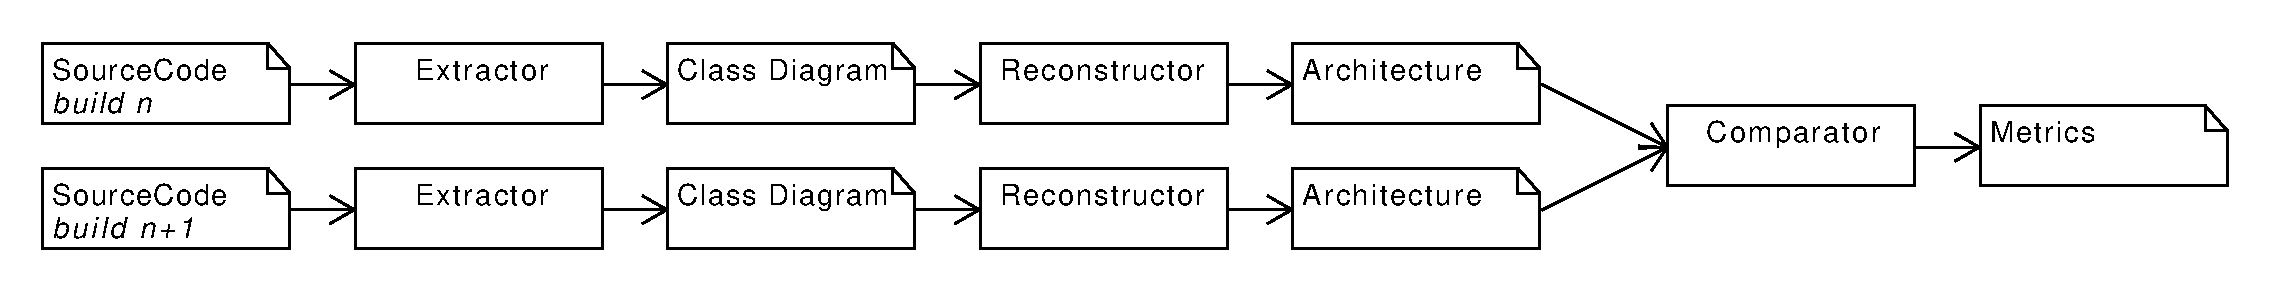
\includegraphics[width=7in]{assets/overview.pdf}
	\caption{Overview of the process}
	\label{overview}
\end{figure*}

\begin{table}
	\caption{Ten Largest Projects under Study}
	\label{tableProjects}
	\centering
	\scalebox{0.9}{
	\begin{tabular}{ | c | c | c | c | c | }
		\hline
		project name & commits & analyzed & range & project type \\
		\hline
		sonarqube & 11590 & 4573 & 1.25y & Code Analyzer \\
		graylog2-server & 8490 & 842 & 4.25y & Log Analyzer \\
		okhttp & 5367 & 1770 & 3.5y & HTTP Client \\
		cloudify & 4984 & 821 & 2.5y & Dev. Framework \\
		structr & 3809 & 1253 & 2.5y & Development App \\
		owlapi & 3238 & 2178 & 3.5y & OWL API \\
		jOOQ & 3196 & 451 & 3y & SQL API \\
		checkstyle & 3029 & 325 & 2y & Code Analyzer \\
		vectorz & 3025 & 46 & 3.5y & Math Library \\
		owner & 2671 & 2099 & 3.5y & Property Files API \\
		\hline
	\end{tabular}
	}
\end{table}


In this study, we have analyzed $159$ projects from the TravisTorrent dataset, which use Java and Maven. In the dataset are $241$ projects which use Java as their main programming language and are built with Maven. We excluded projects, which do not have pushed anything to the master branch or only have one commit, because we cannot compare architectures if there is only one. Then there are some projects where builds or logs could not be retrieved anymore from GitHub and TravisCI or the toolchain was unable to reconstruct the architecture. We are left with $49,531$ commits. An exemplary list of the ten biggest analyzed projects, in terms of unrestricted commits, can be found in table \ref{tableProjects}.

Because the build tool impacts the outcome of the build but not the architecture itself \cite{FailsCorr}, we will limit the study to only one build tool. Although this introduces bias, it ensures consistent results in return. HUSACCT needs the path to the source files, so we can exclude test files and resources. Therefore, we choose the build tool maven with its convention over configuration paradigm. In this way we can be sure where everything is stored in the file structure. This eases the implementation of the class structure extraction. 
Because there are possibly multiple builds for the same commit, we only use the build that builds a certain version of the software first. The following builds are most likely only configuration changes of the CI server and do not introduce new change. Thus, we can ensure that changing configuration does not bias the results. Instead, we compare the changing source code based on the older configuration, i.e. the configuration which is equal to the one of the older build. 

In general, to get an architectural change, we have to follow three steps. First, we need to extract the class structure out of the source code, then we reconstruct the architecture and eventually we take two architectures and compare them with each other to get a change metric (Fig. \ref{overview}). The complete source code and results can be found in our GitHub repository.\footnote{\url{https://github.com/jodokae/cmput663-architecture}}

\subsection{Framework}

\begin{figure}[!t]
	\centering
	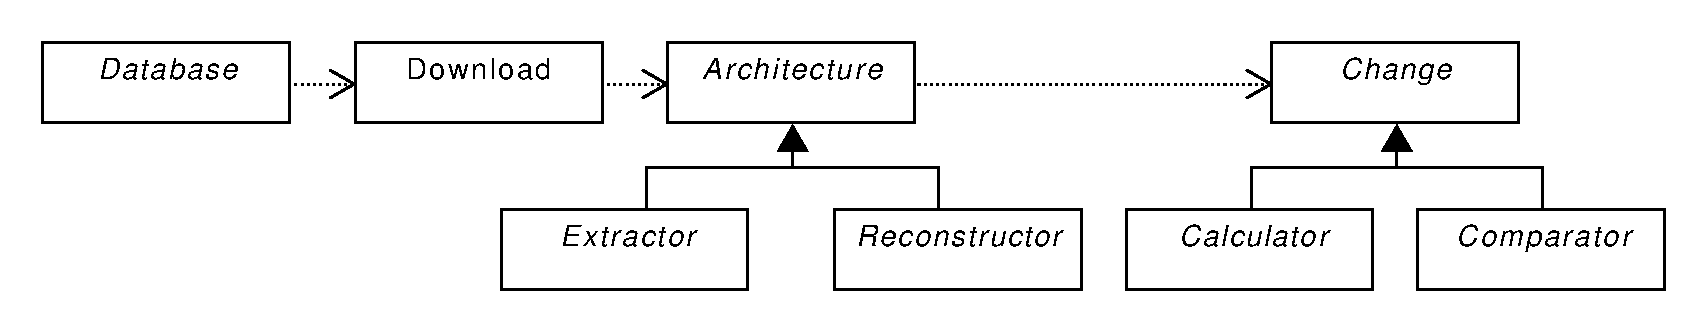
\includegraphics[width=3.45in]{assets/architecture.pdf}
	\caption{Structure of the Framework}
	\label{frameworkStructure}
\end{figure}

We implemented the extraction of the architectural change metrics between two commits using a framework (Fig. \ref{frameworkStructure}). First, the unique commit ID is extracted out of the TravisTorrent database, with which the snapshot can be downloaded from GitHub. 
The ``Architecture'' module is split into two parts, the extraction of the class structure and the reconstruction of the architecture. Intermediate results are saved in a file using the Rigi Standard Format (rsf) \cite{RSF}, because the ARCADE tools rely on this filetype. This filetype saves simple relation triples in the form: type, source, target (see listing \ref{lst1:rsf}). This relational system is easy convertible into a graph structure or a database and stores the modules implicitly in the dependencies. The downside of this format is that the modules cannot be extracted separately but only implicitly while analyzing the dependencies. Fortunately, this is irrelevant for our work.

Then, for every two subsequent commits, we compare the architectures and save the results in a JSON file. With the methodology structured into this framework, the research can easily be expanded with more reconstructors or metric calculators. Therefore, one needs only to implement a new subclass for the changing module, store its result in the Rigi Standard Format and it can be integrated with all existing tools. Doing so, we have combined HUSACCT and ACDC and integrated it with the ARCADE metrics. Similarly, we have implemented the package reconstruction and metrics, so that both ways of computing change can be run independent or simultaneous (Fig. \ref{implToolchain}).

\begin{figure}[!t]
	\centering
	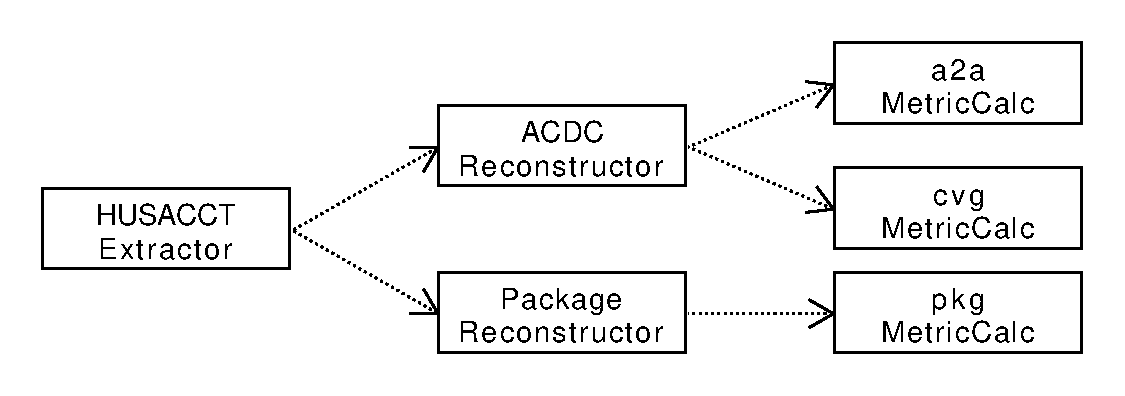
\includegraphics[width=3.45in]{assets/implementedArc.pdf}
	\caption{Implemented tool chain}
	\label{implToolchain}
\end{figure}

\begin{lstlisting}[
frame = single, 
belowskip=-0.8 \baselineskip,
float,
caption=Rigi Standard Format example,
label=lst1:rsf,
columns=flexible
]
subPkg   checkstyle checkstyle.grammars
subPkg   checkstyle checkstyle.gui
contains checkstyle checkstyle.Main
\end{lstlisting}

\begin{table*}
	\caption{Metrics}
	\label{tableMetric}
	\centering
	\begin{tabular}{ | c | l | l | c |  }
		\hline
		Name & Full Name & Description & Builds With Change \\
		\hline
		\#V & Number of Vertexes & Number of changing modules & 1.6\%  \\
		\#E & Number of Edges & Number of changing dependencies & 3.6\% \\
		A. Inst & Absolute Instability & Change of instability for weighted dependencies & 16\% \\
		R. Inst & Relative Instability & Change of instability for unweighted dependencies & 3.4\% \\
		deg & Average node degree & Sum of Edges (unweighted) per module & 3.1\% \\
		a2a & architecture to architecture & number of steps to get from one architecture to another & 67\% \\
		$\text{cvg}_\text{src}$ & cluster coverage (source) & \% of changed modules based on the earlier arch & 39\% \\
		$\text{cvg}_\text{tar}$ & cluster coverage (target) & \% of changed modules based on the latter arch & 40\% \\
		\hline
	\end{tabular}
\end{table*}


\subsubsection{Extraction}

To extract the class structure from the source files, the extractor of the HUSACCT framework is used. For simplicity, and because it is not used in the further analyses, the dependency types are restricted to ``subPkg'', ``contains'' and ``references'', where ``contains'' means that that a package contains a Java type and ``references'' is any dependency between two Java types. The results are then fed into the reconstruction.

\subsubsection{Reconstruction}

Two different reconstruction techniques were implemented. We chose ACDC, because it was evaluated to have one of the best reconstruction accuracy \cite{arcRec-comparison} in comparison with other common techniques. ACDC, in its implementation given in the ARCADE framework, is working directly on the Java byte code. Given that a prominent reason for failing builds is compilation error this is problematic. Therefore, we feed the class structure from the HUSACCT extractor into ACDC and deactivate its own first level extraction.
%TODO Compile Errors

The other technique is the package reconstruction which is often used as ground truth analysis.
This technique looks for the root packages in the system. If there are only a few root packages, it is assumed that the implemented architecture lies a level deeper in the packages. For example, if there is only the ``org.sonar'' as root, this is just the base container and not an architectural element. Therefore, all direct children of this package are considered as modules until there are at least an acceptable number of modules. In this work, 10 was considered the minimum amount of modules needed. This number was chosen with manual sampling over different projects, so that the achieved results were the most consistent with the believed intended architecture. As dependencies all ``references'' edges were considered and added to their respective parent module. This is a valid approach according to Song et al \cite{ArcAsGraph}. 

\subsubsection{Change Metrics}

As explained in Section \ref{sec:Metrics}, the ARCADE metrics a2a and cvg as well as Martin's metrics are used. We calculate the ARCADE metrics on the ACDC architecture. Cvg is calculated twice, one based on the modules of the first version (called source) and one based on the second version (called target).
The coupling metrics are calculated on the package architecture to have some ground truth metrics for comparison. We calculate five package metrics; thus, we have 8 metrics in total (cf. table \ref{tableMetric}).
For every module, the absolute number of incoming and outgoing edges are calculated, the degree of the node (sum over ingoing and outgoing edges), as well as the absolute and relative instability. The absolute instability is based on the absolute number of connections between the modules, i.e. if Module A has only three ingoing connections from Module B, then the afferent coupling is considered three. For the relative instability, the coupling is instead considered one, so it is not measured how tightly connected two modules are, just if they are connected at all.

Since we need the change for the complete architecture, and not for each module, we calculate the mean instabilities and node degree as well as the absolute number of modules (vertexes) and dependencies (edges).

The metrics are then compared pairwise. To compare proportional metrics, like instability, the difference between the values is taken, e. g. if architecture A has an average instability of $30\%$, and architecture B has an average instability of $25\%$, then they are $5\%$ different to each other (Equation \ref{eq:relDiff}). For metrics with absolute numbers, like node degree, the similarity is the proportion of the two values, e.g. A has an average node degree of $8$ and B has $10$, then they are $80\%$ similar, i.e. $20\%$ change (Equation \ref{eq:absDiff}).

\begin{equation} \label{eq:relDiff}
c_{rel}(m_1, m_2) =  \min\{m1, m2\} - \max\{m1, m2\}
\end{equation} 

\begin{equation} \label{eq:absDiff}
	c_{abs}(m_1, m_2) = 1 - \frac{\min\{m1, m2\}}{\max\{m1, m2\}}
\end{equation} 

\subsection{Evaluation}

The calculated metrics are tested for correlation with the build result. This is done in multiple ways. First, the metric is tested against the direct build outcome, then the previous or following $b$ outcomes for $b \in \{2, 3, 5, 10\}$. This means we look for correlation between change in build $x$ and the build result in the builds $\{x, x \pm 1, \hdots, x \pm b\}$. From this, we can see if architectural change correlates to build failures in recent history or near future. 
Then, every metric is converted to a Boolean, which is true if there is a change and false if there is none. This is calculated with a threshold $t$, where everything below $t$ is considered to be no change, and anything above as a change for $t \in \{0.01, 0.02, 0.03, 0.04, 0.05, 0.1, 0.2, 0.5\}$. These values were chosen because most found changes in the dataset were small (Fig. \ref{fig:histograms}) We take these thresholds to find out if small changes affect the amount correlation present in the data. Every comparison which includes no Boolean variables is run with Pearson's correlation test, the others with Spearman's test. 

\begin{figure*}[!t]
	\centering
	\begin{subfigure}{2.3in}
		\centering
		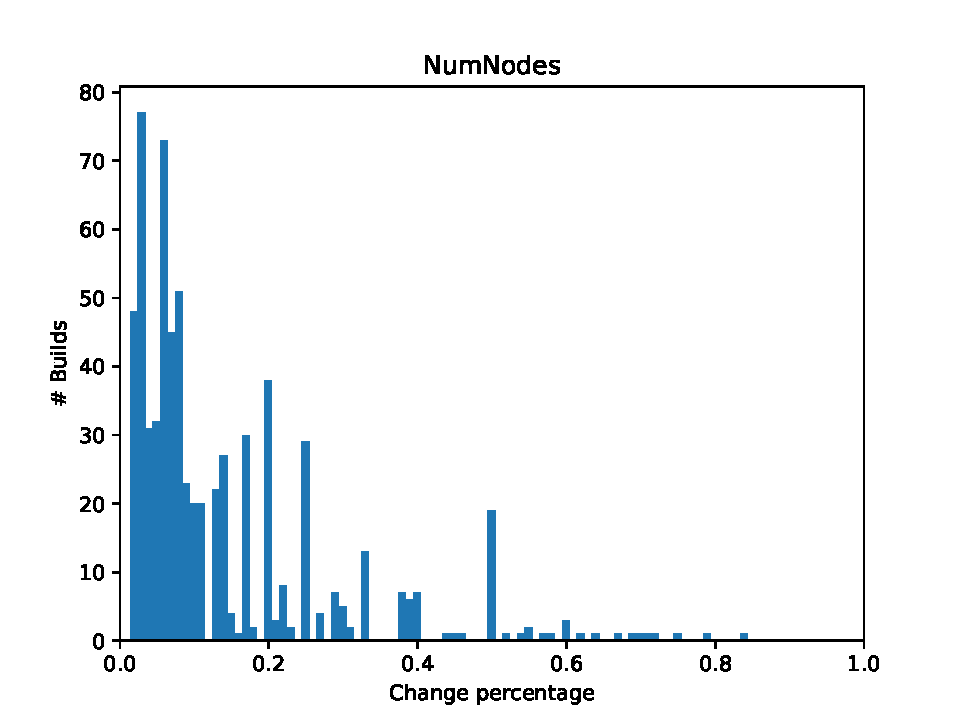
\includegraphics[width=2.3in]{assets/NumNodes.pdf}
		\caption{\#V}
		\label{numNodesHist}
	\end{subfigure}%
	\begin{subfigure}{2.3in}
		\centering
		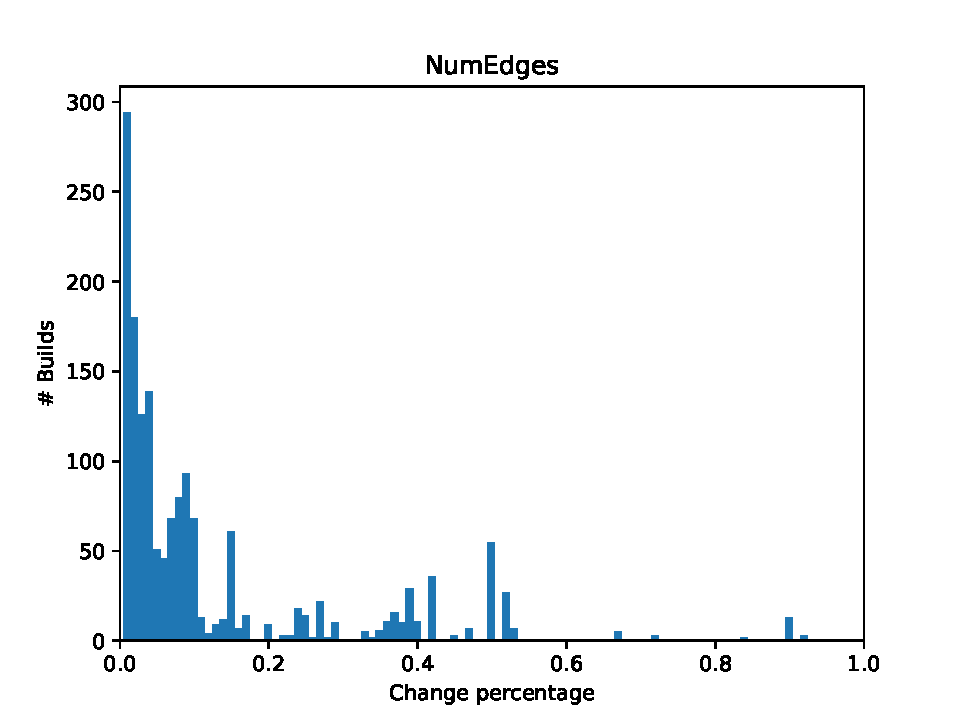
\includegraphics[width=2.3in]{assets/NumEdges.pdf}
		\caption{\#E}
		\label{numEdgesHist}
	\end{subfigure}%
	\begin{subfigure}{2.3in}
		\centering
		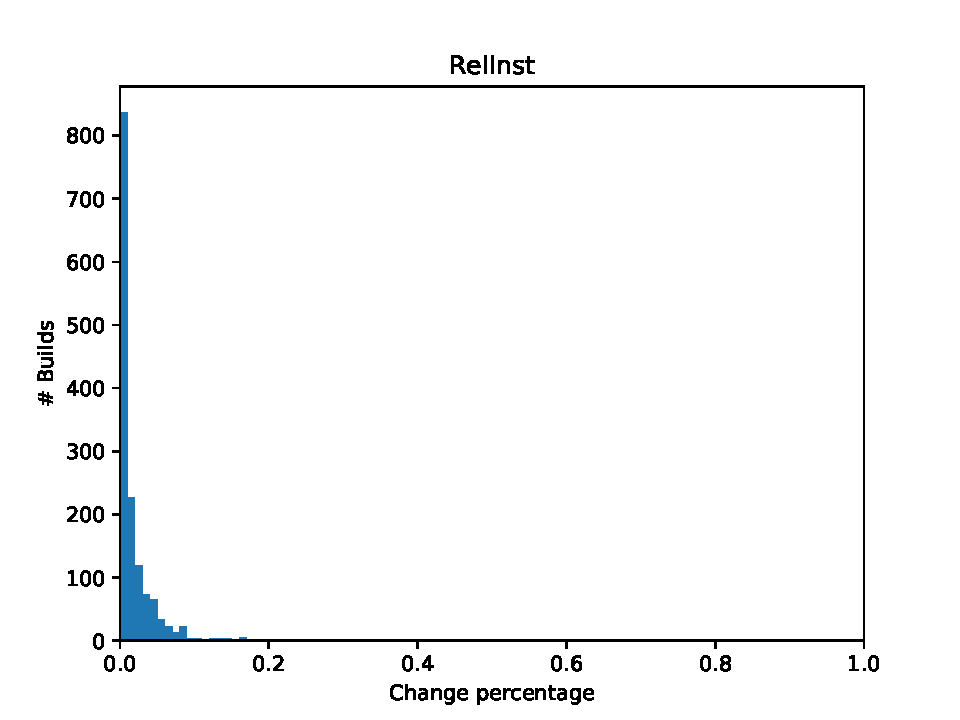
\includegraphics[width=2.3in]{assets/RelInst.pdf}
		\caption{rel. Inst}
		\label{relInstHist}
	\end{subfigure}
	\begin{subfigure}{2.3in}
		\centering
		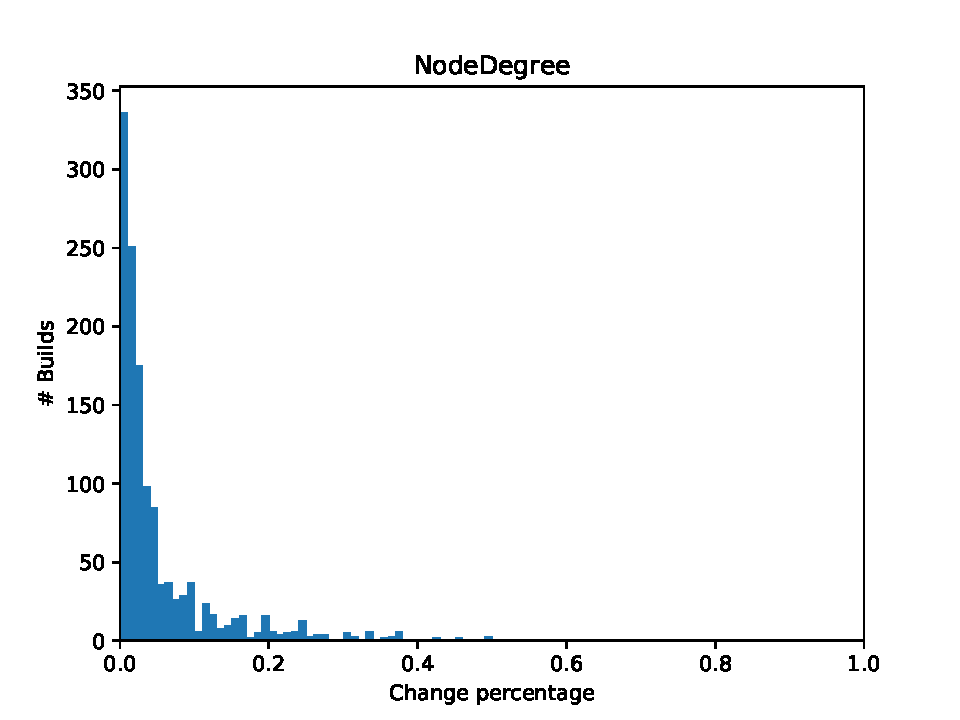
\includegraphics[width=2.3in]{assets/NodeDegree.pdf}
		\caption{deg(V)}
		\label{nodDegHist}
	\end{subfigure}%
	\begin{subfigure}{2.3in}
		\centering
		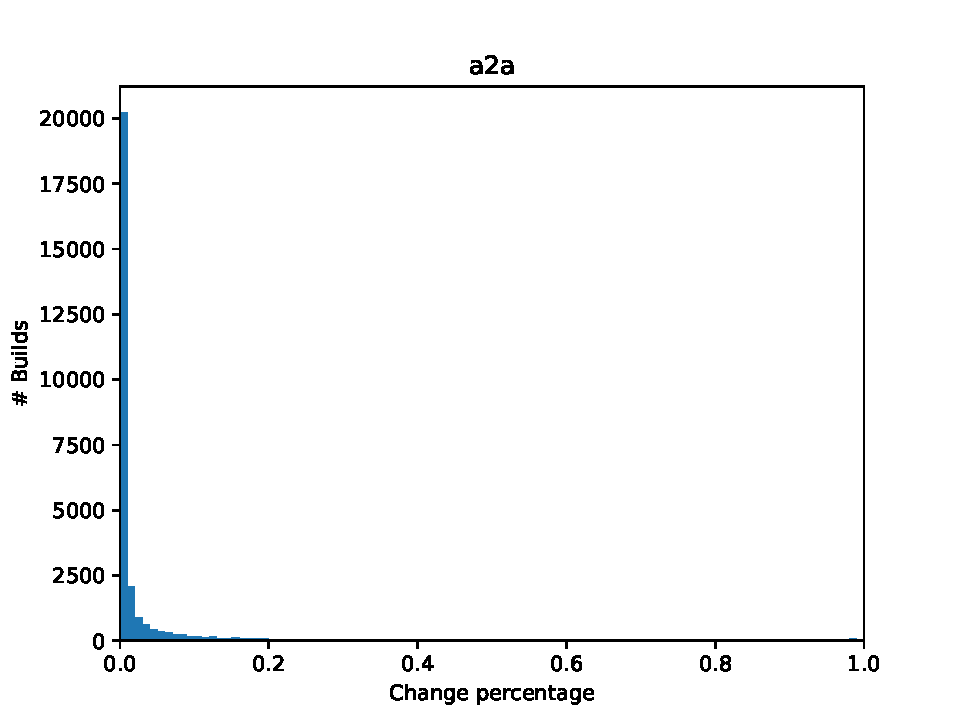
\includegraphics[width=2.3in]{assets/a2a.pdf}
		\caption{a2a}
		\label{a2aHist}
	\end{subfigure}%
	\begin{subfigure}{2.3in}
		\centering
		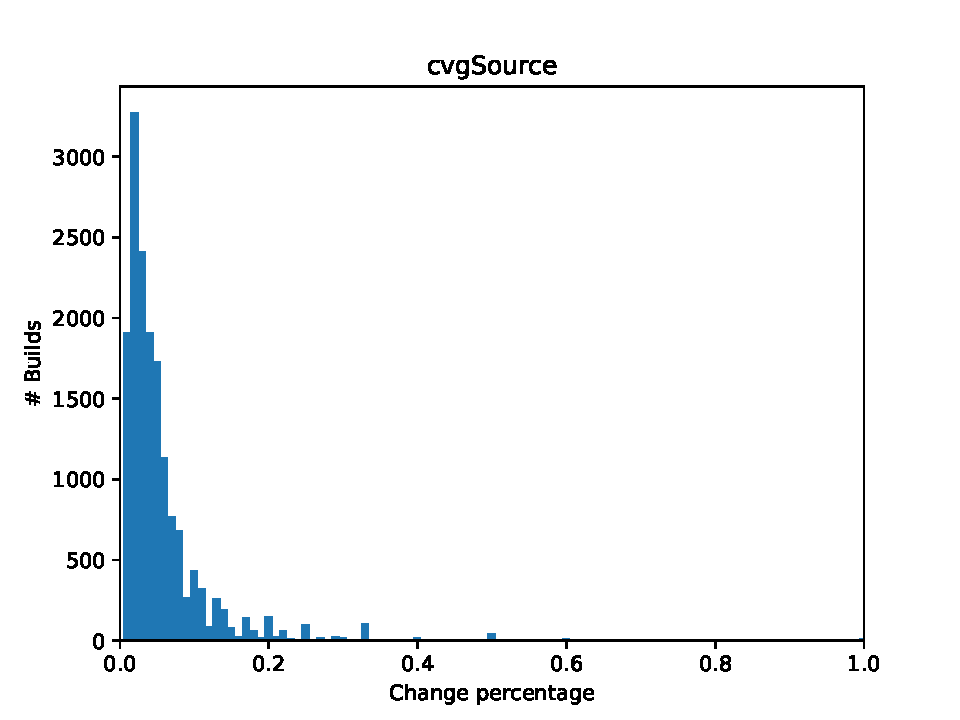
\includegraphics[width=2.3in]{assets/cvgSource.pdf}
		\caption{cvg src}
		\label{cvgHist}
	\end{subfigure}
	\caption{Histograms metric over all projects}
	\label{fig:histograms}
	
\end{figure*}

\section{Results}

%TODO
This section presents the findings with the proposed methodology. First, the projects under study are introduced, then calculated metrics are evaluated and, eventually, the correlation between the metrics and the build outcomes is shown.

\subsection{Studied Projects}

We have studied $49,531$ commits from $159$ projects which use Java Maven. The pass rate is $84.9\%$. Around $10\%$ of the builds failed because of errors before or during the compilation of the software. On third of the errors could be mapped to test errors. The remaining part of the fails were not further separated, but are for example configuration errors or wrong used maven plugins.
The active time of the projects varies. For the ten biggest projects (in terms of number of commits) it is between one and four years of development time, some start at a well-established state (the TravisTorrent dataset starts, for example, at build number 500 for SonarQube), others at build 1 (e.g. Checkstyle). The projects vary in their application field. In the ten biggest projects, there are two code analyzers, three APIs, a web client and an IDE, some for databases, linear algebra or ontologies. Table \ref{tableProjects} gives a detailed list.

\subsection{Metric Evaluation}

p values are all 0 

\begin{table}
	\scalebox{0.85}{
	\begin{tabular}{ | c | c | c | c | c | c | c | c | c | }
		\hline
		& \#V & \#E & A. Inst & R. Inst & deg & a2a & cvg src & cvg tar \\
		\hline
		\#V & 1 & 0.93 & 0.58 & 0.59 & 0.69 & 0.23 & 0.45 & 0.49 \\
		\#E & 0.93 & 1 & 0.63 & 0.71 & 0.83 & 0.25 & 0.51 & 0.55 \\
		A. Inst & 0.58 & 0.63 & 1 & 0.81 & 0.43 & 0.2 & 0.44 & 0.46 \\
		R. Inst & 0.59 & 0.71 & 0.81 & 1 & 0.56 & 0.22 & 0.48 & 0.52 \\
		deg & 0.69 & 0.83 & 0.43 & 0.56 & 1 & 0.18 & 0.41 & 0.46 \\
		a2a & 0.23 & 0.25 & 0.2 & 0.22 & 0.18 & 1 & 0.38 & 0.37 \\
		cvg src & 0.45 & 0.51 & 0.44 & 0.48 & 0.41 & 0.38 & 1 & 0.91 \\
		cvg tar & 0.49 & 0.55 & 0.46 & 0.52 & 0.46 & 0.37 & 0.91 & 1 \\
		\hline
	\end{tabular}
	}
\end{table}


We have extracted 8 architecture change metrics. Most builds show no change (table \ref{tableMetric}). This is to be expected, since most changes in the system should not be architectural changes. 
%TODO Confirm with new data
Only a2a has more changing builds than non-changing builds. But then, most of these changes are really small, as shown in Fig. \ref{a2aHist}. In other metrics, most changes are quite small as well, with only few big architectural changes (Fig. \ref{cvgHist} and \ref{numEdgesHist}). This seems usual, because we assume that the architecture does not have big changes that often.

%TODO Confirm p Values
%TODO Maybe make table with all values
In table \ref{tableMetricCorr} the correlation between the metrics is shown. All p values were equal or close to 0. Most metrics are highly correlated, and all show some degree of correlation ($>0.2$). This gives the indication that all metrics are truly an indicator for architectural change if we assume that at least one of them is. This strengthens the confidence in the chosen tool chain. 
%TODO Manual Sampling - Check some values

\subsection{Correlation}

Most found correlations, with a p-value under $5\%$, were between $0.1$ and $3\%$. Only some metrics show a higher correlation around $9-11\%$. The threshold controls how many previous or following builds were considered, had no significant impact. The highest correlation found was for cvg, regardless of source or target, with a change threshold of $0.0$, i.e. every little change was considered as change (Fig. \ref{cvgPlot}). But even the best correlation was only $11\%$. 

The small p values show that we have a statistical significant relationship between change and build outcome. But this correlation is so small for most metrics, that we cannot conclude this as a meaningful impact. Because taking the smallest changes into consideration increases the correlation coefficient, and the threshold for previous and following builds had no significant change on that coefficient, it must be assumed that the stronger correlations could be noise. Because the strongest correlation was found with the cvg metric, which works inside of the modules, the possible correlation is within the modules not between them. Furthermore, over all correlations, the tendency was towards a positive value (min: -0.03), which shows, if there truly is a correlation, then change is occurring more often around non failing builds, whereas a static architecture shows in the near of failing builds. 

\begin{figure}[!t]
	\centering
	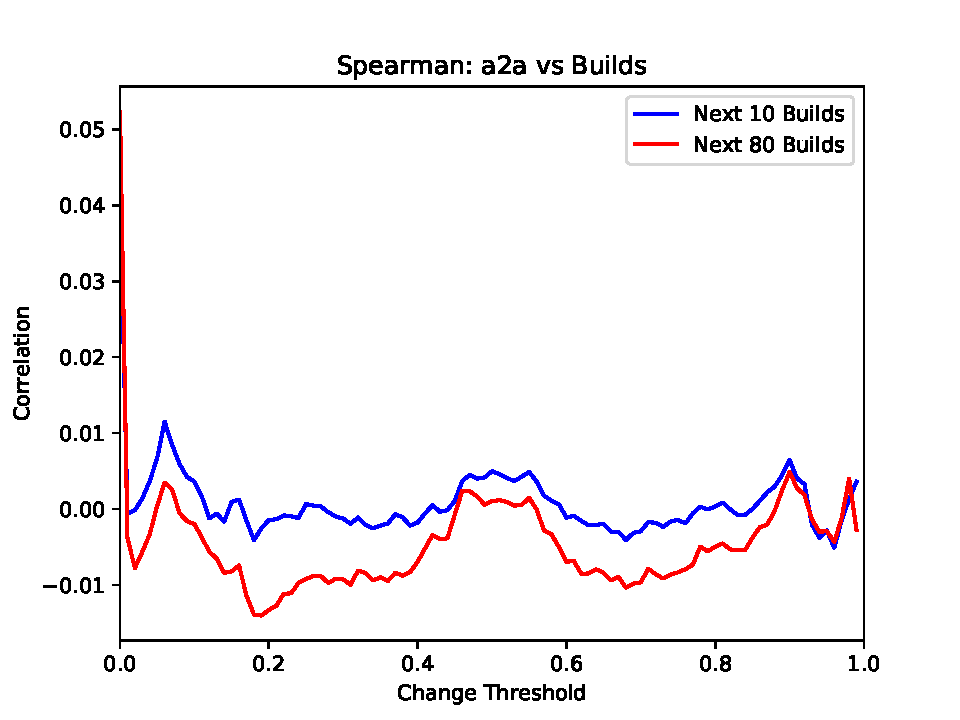
\includegraphics[width=3in]{assets/a2aCorr}
	\caption{a2a vs next ten and eighty builds over different change thresholds }
	\label{a2aPlot}
\end{figure}

\begin{figure}[!t]
	\centering
	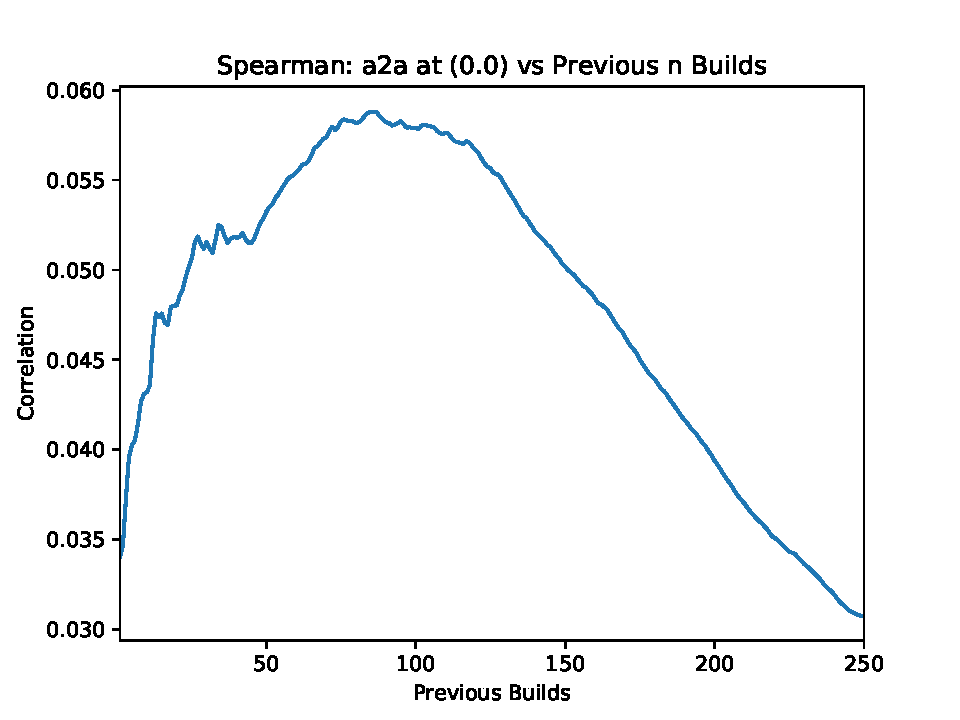
\includegraphics[width=3in]{assets/PrevN}
	\caption{a2a vs previous n builds over 0.0 threshold }
	\label{a2aPrevN}
\end{figure}

\section{Discussion}

While checking ten big Java projects, no significant correlation between architectural change and build results was found. Apart from there actually being no correlation, there could be various factors influencing this result. 

First of all, only ten projects, although from different domains, were evaluated. Despite having projects which start at build one, the number of failing builds was relatively small. It is possible that the missing connection between architecture and build results lies in the possibility that all considered projects have a well thought-through architecture and do change it in a way that in produces problems. This can be backed up by the fact that most found changes are below a threshold of $10\%$ change. It will be interesting to see if projects with a more unstable architecture show more failures. In this research, no significant change cross-projects was found but a large-scale analysis between more projects could be done in future. 
%TODO REVAMP this

It is also possible, that the problems which are produced by architectural change are not transferred into build results but to a different level, e.g. (1) code coverage or (2) number failed tests. Unfortunately, the dataset does not give the opportunity to check for those, because they are (1) not reported and (b) have missing values in around $20\%$ of the builds. The fact that software architecture is important is common knowledge. We showed that it changes over the lifetime of a project. However, it remains unknown how architecture change affects the progress of the development process.

As Garcia et al. \cite{arcRec-comparison} show even the best recovery techniques have problems detecting the true architecture. Therefore, it is possible that HUSACCT and ARCADE are not the right tools for the research question. This problem was addressed since we consider multiple recovery techniques and rely on studies which evaluate ARCADE as being one of the most accurate recovery tools. The produced metrics highly correlate, which strengthens the claim that the change detection is working as intended. Still, it is possible that the chosen metrics are not the best set. Because they correlate so strongly, they are a weak feature set if one would try to use machine learning techniques to predict the build outcome. For this, a broader set of metrics is necessary. 

In the future, more metrics and extractors should be added to the framework. Then, it is necessary to broaden the research to find better quantitative data which show problems in the software that could be caused by bad or changing architecture. Because this work introduces an easy expandable framework, this should be possible with little to no effort.

\section{Conclusion}

While analyzing over $20,000$ builds from $10$ different Java Maven projects from various domains, we could not find any significant impact of architectural change on build outcome.
We approached this result through an easily expandable framework to recover the architecture from the builds using one extractor, two reconstructors, and three metric sets based on previous researches. In total, $8$ metrics were tested for correlation in $6$ different scenarios including the previous and following builds. 

The hypothesis that architectural change impacts CI build outcomes at or near the change was rejected. The highest correlation found was around $11\%$ and would imply that change leads to fewer failures. This could just be noise, due to the well-established nature of the studied projects, or that is no correlation between architectural change and build outcome. 

We conclude that change does not impact the build outcome and, thus, the research questions have to be changed. Since it is known that the architecture impacts the development, other quantitative features must be found to measure the impact. We propose to extend the measured metrics, because we believe that one metric cannot explain the impact alone, and search for correlation in more nonfunctional metrics, like code coverage or development pace.
The built framework can be efficiently adapted for the new questions through extracting more facts out of the code using various tools. 

\bibliographystyle{ACM-Reference-Format}
\bibliography{literature}

\end{document}
\grid
